This chapter deals with the collaboration and process in the project. We introduce the initial background and motivation of the project. Afterwards we introduce the project management work and collaboration within the project. We present the project management tools we used, describe our experience and evaluate the used tools.
Finally, we cover the major collaboration issues we had to face during the project. Furthermore we reflect on the process and collaboration and describe our learning outcomes.

%---

% --- INTRODUCTION GLOBAL COLLABORATION ---

%\section{Introduction} %OBSOLETE
%Trust is one of the major keys for succes of teamwork \todo{929eng - page 11}.

%With the increase of trust within a project team, the team members will work more effectively \todo{929eng - page 9}.

%Trust within a project team grows with the communication. It is known that besides verbal especially non-verbal communication - like vocal interaction and body language - influences communication\footnote{929eng - page 7}. Global-distributed project teams are often limited in communication options. Accordingly building up trust within a global-distributed project team via non face-to-face communication is more challenging than within a local project team.

%Physical perception of members within a project team, makes the members more aware of a collective, which can raise the commitment to the project team and the project. As this also can be difficult to arrange for a global-distributed project teams, it has to come back on other approaches to develop a corporate feeling and affiliation for each member.

%The paper "Communication and Trust in Global Virtual Teams"\todo{reference} looks into if trust can even exist within teams, which are only using virtual communication.

%---

% ---BACKGROUND ---

\section{Background information of the Project Team}
\label{sec:background}

The project team consists of two groups of students. One group is from Strathmore University located in Nairobi (Kenya). The other group is from the IT University (ITU) in Copenhagen (Denmark). The project team agreed on to name the two groups "Team Kenya" for the student group from Strathmore University and "Team ITU" for the student group from ITU. This helped to address each group in meeting reports, emails and conversations.

In the following paragraphs the background information for this project from both groups are introduced. The information explains the motivation and contribution of each group in the project and is used in arguments for why certain decisions were made and issues arise.

% --- TEAM ITU ---

\subsection{Team ITU}
\label{sec:team_ITU}

Team ITU started with four members, which are all in the Masters programme "Software Development and Technology (Software Engineering)" of the ITU\footnote{In the beginning there were five members, but one left the project after two weeks, because he changed to another project and project team. This did not have an impact on the work as it was in the early stage of the project.}. The members are from three different countries: Lithuania, Germany and Denmark\footnote{Although there are minor differences between the nationalities, which could have an influence on the team work, we will not go into this, because it is out of scope for this report.}. The communication language within Team ITU is English, which is not the mother tongue of any of the members. Two of the members of Team ITU already collected some negative experience with previous global collaboration projects. They experience that the other groups in their previous global collaboration projects did not put much effort into the projects, so that they and their local team had all the workload. Therefore there have been some prejudices at the beginning of the cooperation. The members of Team ITU met each other the first time on the 27.8.2013.

The students of Team ITU have to complete the project under the course "Global Software Development Project", which is mandatory for their masters programme. The requirements and deadlines for the project are given in the course base from ITU and by the advisor of the project. The course is rated with 15 ECTS points, which corresponds to approximately 20 hours per week per student. The students of Team ITU have to hand in this report as a mandatory requirement.

As the course for the Team ITU started in late August and the project team and topic was already known, Team ITU already started with the project work before Team Kenya. Team ITU and their advisor did not know when they would get the contact details from the student group in Kenya, so the advisor recommended already initializing the project and doing some research and thoughts on the project.

At the beginning Team ITU had received a different project topic by the advisor. The topic of the first project was "Vector Shooter"\footnote{In this project a game had to be developed, in which the calculation of a vector - based on an image - had to be made. The image should contain a person, who uses his hands to demonstrate a vector by taking a position like he uses a bow and arrow. The requirement was to use webcams, to capture the image, and to use RaspberryPis to detect the hands of the person and to calculate the vector. Furthermore, an Android application should be included in the program.}. Team ITU put some thoughts into the project and spent time on defining the program, which they wanted to develop\footnote{Team ITU planned to develop an individual cannon game with an appropriate concept for a global collaboration project.}.

After three weeks the advisor had to change the topic of the project due to the collaboration with Strathmore University. Only one student from the Strathmore University was interested on the project "Vector Shooter". Team ITU could have spent time and effort in convincing the other students from Strathmore University to do the project "Vector Shooter". Despite frustration, in consideration of the given deadline of the course and on recommendation of the advisor, Team ITU decided to not take this option.

Team ITU received the project topic and the contact details of the members of Team Kenya on the 17.9.2013. A collaboration between the student groups did not start before this date.

% --- TEAM KENYA ---

\subsection{Team Kenya}
\label{sec:team_Kenya}

In the beginning Team Kenya consists of three members, which are all in the Masters programme "Telecommunication and Innovation" of the Strathmore University. The members are all from Kenya. The official languages in Kenya are English and Swahili. The members of Team Kenya met each other the first time on the 1.10.2013 (--> Appendix \ref{app:appendixB}: \hyperlink{GSD20131001.1}{Global Meeting Report 1.10.2013 Page 1}). One member had to leave the group in the last third of the project due to workload of other projects and obligations (--> Appendix \ref{app:appendixB}: \hyperlink{GSD20131126.2}{Global Meeting Report 26.11.2013 Page 2}).

The department, which is responsible for the masters programme "Telecommunication and Innovation", wants to convince the school management from Strathmore University to invest into the technology and idea of the project to improve environmental conservation. Therefore this collaboration project was initiated. (--> Appendix \ref{app:appendixB}: \hyperlink{GSD20131203.2}{Global Meeting Report 3.12.2013 Page 2}).

For the students from Team Kenya the project is not included in any mandatory course and is completely voluntarily. The students from Team Kenya spent their free time on this project, as they did not have reserved time for thi sproject like Team ITU had (--> Section \ref{sec:team_ITU}). There are no mandatory requirements or deadlines, which the Kenyan students have to achieve, except that they have to create documentation for their advisor to prove the progress of the project (--> Appendix \ref{app:appendixB}: \hyperlink{GSD20131119.2}{Global Meeting Report 19.11.2013 Page 2}). The motivation for the Kenyan students to participate in this project is on the one hand to support the environmental thought and on the other hand to use this project work as basis for their master thesis (Email 10.12.2013 \todo{Add refernce}).

%---

% --- PROJECT MANAGEMENT ---

\section{Project Management}
\label{sec:project_management}

% --- PM APPROACH ---

\subsection{Approach}
\label{sec:approach}
There are several approaches how you can perform project management for software development projects. It is often distinguished between the traditional approach and the agile approach in project management.

The traditional approach in project management is dividing the project into distinguished phases, which are planned in advance. The phases are run sequentially. Theoretically, once a phase is complete it will not be revisited. This structure is also known as waterfall model in software development\footnote{Waterfall model: \url{http://en.wikipedia.org/wiki/Waterfall_model}}.
The problem with this traditional approach is that it is not very flexible for unpredictable events. Furthermore, clients are often unable to state all requirements in the beginning. A change of a requirement or the adding of additional requirements during the project can have a major impact on the project plan and is often embedded in an extensive change management process.

%NOT USED:
%The traditional approach plans the project in the beginning. All requirements and ressources are collected and planned in the beginning of the project to build up a project plan, which containes a detailed project tasks and milestones. These pre-planned project tasks are then worked off during the project. The project manager can keep track and report the progress of the project by comparing planned and actual progress.

The agile approach is in general more flexible than the traditional approach, especially when it comes to requirements and unpredictable events. The idea of an agile approach is to have many iterative planning and development cycles. The approach supports quick results, which are constantly improved by involve the client actively in the project progress. An agile approach does not intent to have a completely pre-planned process like in the traditional approach. In software development projects an agile approach is preferred due to its advantages. A popular agile project management framework is Scrum\cite{scrum}.

As the course for the Team ITU started in late August and they already met each other, Team ITU already started with a project management technique. This was already established when Team Kenya got into the project.

Team ITU tried to follow an agile project management approach, because it is more flexible, which was important due to the fact, that Team ITU did not knew the student group from Strathmore University neither their skills nor their requirements on this project. Moreover an agile project management approach is known for being more suitable for software development projects\cite{project_management_approches}.

Team ITU planned to merge Team Kenya into their project management approach, because they did not come up with a different approach on how to organise the project. Team ITU asked for feedback or other suggestions according to project management methods and tools, but Team Kenya did not react at all or agreed with the suggestions of Team ITU. Therefore Team ITU assumed that Team Kenya is fine with the project mangement approach.

In general Team Kenya was very reticent in project management topics, although one student from Team Kenya seemed to be very interested in the project management and global collaboration challenges (--> Motivation-Sheet in Appendix \ref{sec:Motivation_Sheet}). In the end it also turned out, that the one Kenyan student, who was the most interested in project management and global collaboration, left the project due to other obligations. This did not had a major impact on the project, because the student in question did not interacted that much within the project.

Team ITU considered introducing Scrum to the project. However, due to the inexperience and non-knowledge about this framework in both teams, this idea has been dropped. For Scrum it is necessary that every project team member knows the concept. Accordingly, each team member would need to learn Scrum, which in turn would have taken ressources from the implementation.

It turned out that Team ITU was not able to use an agile project management approach properly. An agile approach requires a strong collaboration between the project team members and healthy communication. It is also essential, that the project team members have the needed competencies and that everyone support the project\cite{agile_project_management}. This project had issues according to communcation, cooperation and skills(--> Section \ref{sec:issues}), which made it rather difficult to use any kind of project management approach.

%---

% --- PROJECT ORGANISATION ---

\subsection{Project Organization}
\label{sec:organization}
Team ITU suggested to split up the project tasks, such that the skills are best utilized within the project and such that Team ITU is not dependend on Team Kenya. The suggestion was that Team Kenya focusses on the Android Application part and Team ITU on the occupancy detection and prediction part.

The Android Application part includes the definition of the functionlity of the Android Application and the definition of requirements for the Android Application towards the server. The occupancy detection and prediction part contained image processing on RaspberryPis, development of a prediction model and setting up the server. Although the tasks were split each group was welcomed to make suggstions or give feedback on the work of the other group.

According to the Skill- and Preference-Sheet (--> Appendix \ref{sec:Skill_Preference_Sheet}) the members of Team Kenya felt the most comfortable with the Android Application part. Team ITU was less interested and skilled in Android Applications and had a greater interest in the occupancy detection and prediction part of the project. Furthermore, Team Kenya did not have access to RaspberryPis until then and it was uncertain if they will have access in the near future\footnote{It turned out that Team Kenya received access to RaspberryPis on the 26.11.2013 (--> Appendix \ref{app:appendixB}: \hyperlink{GSD20131126.2}{Global Meeting Report 26.11.2013 Page 2})}.

In addition the occupancy detection and prediction part was not depended on the Android Application part. Since Team ITU already experienced a lack of communication, cooperation and initiative (--> Section \ref{sec:issues}) within the collaboration with Team Kenya, they had a big interest in being independent from Team Kenya as much as possible.

Both groups agreed on the suggested split of tasks in the meeting on the 24.10.2013 (--> Appendix \ref{app:appendixB}: \hyperlink{GSD20131024.2}{Global Meeting Report 24.10.2013 Page 2}).

Team ITU split up their project tasks within their group such that different roles could be formed. Therefore each member of the Team ITU had a topic to focus on and felt integrated into the team. The roles were not sharply separated.

The following roles describe the major responsibilities within Team ITU:
	\begin{itemize}
		\item Image Processing Developer
		\item Prediction Model Developer
		\item Server Developer
		\item Collaboration master
	\end{itemize}

Also Team Kenya split up their duties into two major responsibilities (--> Appendix \ref{app:appendixB}: \hyperlink{GSD20131119.1}{Global Meeting Report 19.11.2013 Page 1}):
	\begin{itemize}
		\item User Interface Developer
		\item Application Logic Developer
	\end{itemize}

%---

% --- PROJECT MANAGEMENT TOOLS ---

\subsection{Project Management Tools}
\label{sec:tools}
In the following subsections we introduce the different project management tools, which were used during the project. The experience gained with these tools from the perspective from Team ITU are presented. In addition we describe how Team ITU reacted on certain incidents.

% --- MEMBER PROFILES ---

\subsubsection {Member profiles}
\label{sec:member_profiles}
Team ITU suggested to come up with some member profiles of each project team member to introduce each other in the beginning of the project. The intention of the member profiles was to set the first steps for building up trust within the distributed project team. The project team members could recognise the members as individual persons with own personalities and different backgrounds in the beginning. The profile members should also preclude misunderstandings, for example according to the genders and how to address a person.

One member of Team Kenya followed the suggestion in the beginning. The other two members provided their member profiles three weeks after Team ITU reiterated the request.

Because Team ITU did not receive the member profiles of all students from Team Kenya in the beginning, a first disappointment on the side of Team ITU could be noted. Team ITU already waited since end of August to meet the Kenyan group, with whom they supposed to work with. There was high curiosity on the side of Team ITU, which was not satisfied by Team Kenya. This probably already led to a higher mistrust right fom the start, as two members from Team ITU, which already collected some negative experience with previous global collaboration projects, felt reassured.

% --- SKILL AND PREFERENCE AND MOTIVATION ---

\subsubsection {Skill-/Preference- and Motivation-Sheet}
\label{sec:skill_sheet}
To see where the strengths, weaknesses and motivations within the project team are, Team ITU came up with a Skill-/Preference-Sheet and Motivation-Sheet. The Skill- and Preference-Sheet focusses on the technical concerns like programming languages, version control tools, database- and other technologies. So when a skill in a technology is purely pronounced within the project team, the most preferred technologies can be considered. The Motivation-Sheet, on the other hand, focusses more on the different project work tasks and topics. With this information the roles within the project can be split up, so that every member is the most satisfied and therefore more motivated.

Every project team member was encouraged to fill out these tables. Also here Team ITU had to reiterate the request. The results can be seen in the Appendix \ref{sec:Skill_Preference_Sheet} and \ref{sec:Motivation_Sheet}.

The outcome of these tables also influenced some decisions in the project. For example, the decision of which programming languages Team ITU choose to benchmark was based on this (--> Section \ref{sec:benchmark}). Also the choice of database technology and which version control system to use for the source code is based on the Skill-/Preference-Sheet. It also pointed out the possible roles of each project team member within the project (--> Section \ref{sec:organization}).

In the result it can be noticed that image processing, prediction models and RaspberryPis were quite unknown amongst the project team members. Therefore each project team member was encouraged to do some research on these topics in the beginning.

% --- CALENDAR ---

\subsubsection{"Out-of-Office"-Calendar}
Because every project team member had different obligations besides the project, Team ITU came up with an "Out of Office"-Calendar, in which every project team member could publish for example exams, other hand-ins or other unavailability. The motivation of this calendar was to allow for better planning of meetings and assignments during the project. The problem was that no one really looked into this calendar except in the beginning of the project or when a certain issue aroused. The "Out-of-Office"-Calendar can be seen in the Appendix \ref{sec:Calendar}.

So it was noticed by Team ITU that Team Kenya as well as Team ITU had some exams in October. This influenced the project plan according to when to probably start the implementation phase. In the first half of November Team Kenya had a second exam phase. This was not correctly mentioned in the calendar, so Team ITU was not aware of this situation in the beginning. Team ITU got informed of the exam phase by Team Kenya in a meeting, when Team Kenya excused themselves for the non-fulfillment of agreed assignments (--> Appendix \ref{app:appendixB}: \hyperlink{GSD20131112.2}{Global Meeting Report 12.11.2013 Page 2}).
%This led to amazement and disappointment on the side of Team ITU. Team ITU wondered why Team Kenya even agreed on the assignments the week before, when they knew that they probably do not have the time to fulfill these assignments. Team ITU expected that Team Kenya communicates such situations before they happen.

% --- MILESTONE PLAN ---

\subsubsection{Milestone plan}
\label{sec:milestone_plan}
Team ITU chose to create a very rough milestone plan to have an eye on the deadline given by ITU. A detailed milestone plan would contradict the idea of the agile project management approach. Team ITU did not know Team Kenya, their skills and requirements in the beginning and a detailed milestone plan probably would have been rescheduled several times. In the milestone plan Team ITU roughly pointed out important deadlines for specific parts of the project.

\begin{table}[tb]
	\centering
	\begin{tabular}{ |  p{4cm} |  p{6cm} | l | l |}
    		\hline
   		Milestone & Description & Planned & Achieved \\ \hline
    		First Global Meeting & Introduction session with Team Kenya to get to know each other and sharing requirements and expectations of the project & 01.10.2013 & 01.10.2013 \\ \hline
    		Final definition of Requirements and Roles & Get all the main requirements together and splitting up the project tasks & 31.10.2013 & 03.12.2013 \\ \hline
    		Finishing Prototype & A complete prototype of the product & 01.12.2013 & 15.12.2013\\ \hline
		Report & A complete final report of the project & 13.12.2013 & 16.12.2013\\ \hline
	\end{tabular}
	\caption{Milestone Plan}
	\label{tab:milestones_table}
\end{table}

As it can be seen in table \ref{tab:milestones_table} the planned deadlines were mostly not achieved in time. The most significant difference between a planned and a achieved date can be seen at the second and third milestone, which contained a final defintion of requirments and roles and the development of a prototype. The reason for this is on the one hand that Team ITU was too optimisitic in the planning process of these milestones, as they assumed that the members of Team Kenya have the same work pace and working experience like they have. Furthermore the milestone plan was probably not properly introduced and discussed with Team Kenya. On the other hand Team ITU could not encourage Team Kenya enough to do their part of the project in time or the results were not satisfactory enough, such that Team ITU could work with it. In consequence several iterations and new requests had to be made from Team ITU to Team Kenya, which slowed down the project progress a lot. Team ITU was to patient in the end, because they still hoped that Team Kenya will get a better drive after their exam period as Team Kenya make Team ITU believe.

Figure~\ref{fig:milestones} shows the milestone plan, which was planned in the beginning of the project.

	\begin{figure}[tb]
		\centering
		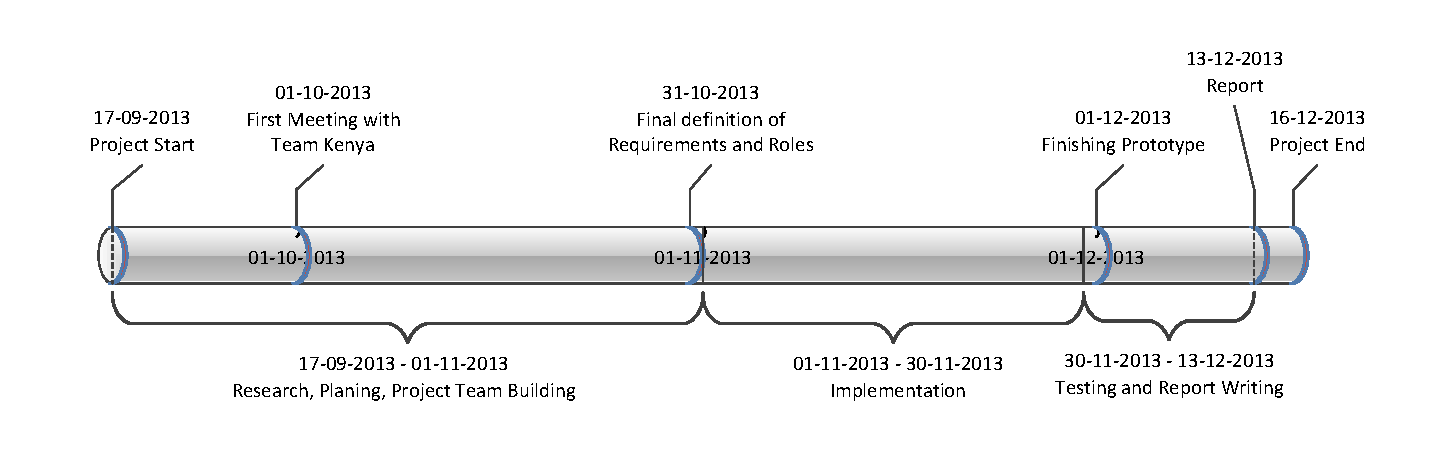
\includegraphics[scale=0.7]{collaboration/Milestones}
		\caption{Milestone Timeline}
		\label{fig:milestones}
	\end{figure}

The milestone plan was mostly a guideline for Team ITU, because they had a deadline in contrast to Team Kenya. Team ITU shared the planed dates for half of the milestones with Team Kenya as they agreed to go with the deadlines from Team ITU. (--> Appendix \ref{app:appendixB}: \hyperlink{GSD20131024.1}{Global Meeting Report 24.10.2013 Page 1}) These shared milestones were according to when to finish the prototype and when to hand-in the mandatory final report.

% --- INTERNAL MEETING ---

\subsubsection{Internal weekly meeting (Jour-Fixe)}
\label{sec:internal_meeting}
Team ITU agreed on having an internal weekly face-to-face meeting to update each other on the current progress, to discuss occuring topics, make decissions, work together and assign each other new assignments till the next meeting. Furthermore Team ITU also met with their advisor to check if they are on the right track. The concept of the weekly meeting equates to the concept of a Jour Fixe\cite{jour_fixe} or a Daily Scrum\cite{scrum}.

There was a constant agenda for the meeting:

	\begin{enumerate}
		\item Status update of each team member
			\begin{enumerate}
				\item What has each group done during the past week according to the project?
				\item Which achievements were made?	
				\item Which problems occurred?
				\item Any other news
			\end{enumerate}
		\item Discussions and Decisions (the topics in this section varied weekly according to the current progress)
		\item Meeting with advisor	
		\item Assignments
	\end{enumerate}

This constant agenda gave some structure to the project. The team members knew what to expect from the meeting and where they can place their concerns.

The members of Team ITU were mostly fully represented in the internal weekly meeting. 

% --- GLOBAL MEETING ---

\subsubsection {Global weekly meeting (Jour-Fixe)}
\label{sec:global_meeting}
Team Kenya and Team ITU agreed on having a weekly Chat-Meeting to update each other on the current progress, to discuss occurring topics, make decisions and assign each other new assignments till the next meeting, just like the weekly internal meeting.

The supporting tool for the meeting was Skype. Both teams agreed on to use Skype instead of Google Hangout. In the initial meetings the groups tried to use a video and audio conference call both in Skype and in Google Hangout. Due to connection problems, especially with several clients, and difficulties to understand each other, it was suggested by Team ITU to use the chat option and using the audio conference call option only when it was needed. This was for example to explain something in detail.

The meeting took place every Tuesday afternoon/evening. According to a Doodle-Survey (--> Section \ref{sec:surveys}) all project team members could reserve this time for the project meeting. Each group could make a suggestion for the agenda. Therefore only Team ITU prepared an agenda, which was structured in the following way:

	\begin{enumerate}
		\item Status update of each group
			\begin{enumerate}
				\item What has each group done during the past week according to the project?
				\item Which achievements were made?	
				\item Which problems occurred?
				\item Any other news
			\end{enumerate}
		\item Discussions and Decisions (the topics in this section varied weekly according to the current progress)
		\item Assignments
	\end{enumerate}

It can be noted, that the structure for the agenda of the global meeting is similar to the agenda of the internal meeting. This is because the structure was already proofed by Team ITU before the global collaboration started and was considered to be suitable by all members from Team ITU. Although it was offered to Team Kenya, they never made alterations to the agenda.

After the first few meetings Team Kenya and Team ITU agreed to prepare the status update in advance, because it took quite a while for each group to present their status updates in the Skype chat. Unfortunately Team Kenya did not comply with this agreement except in the last meeting, where none of the Kenyan students could attend due to other obligations or internet connection problems (Table~\ref{tab:global_meetings}).

\begin{table}[htb]
	\centering
	\begin{tabular}{ | l |  p{2.5cm} |  p{2.5cm} |  p{3cm} |  p{3cm} |}
    		\hline
   		Global Meetings & Attendance Team ITU &  Attendance Team Kenya & Prepared Status update Team ITU & Prepared Status update Team Kenya\\ \hline
    		01.10.2013 & 4 & 1 & no & no \\ \hline
    		24.10.2013 & 4 & 2 & no & no \\ \hline
    		31.10.2013 & 3 & 2 & no & no \\ \hline
    		12.11.2013 & 4 & 2 & no & no \\ \hline
    		19.11.2013 & 4 & 2 & yes & no \\ \hline
    		26.11.2013 & 4 & 1 & yes & no \\ \hline
    		03.12.2013 & 3 & 1 & yes & no \\ \hline
    		10.12.2013 & 4 & 0 & yes & yes \\ \hline
	\end{tabular}
	\caption{Attendance and prepared status updates of the global meetings}
	\label{tab:global_meetings}
\end{table}

As it can been seen in Table~\ref{tab:global_meetings} almost every meeting took place. The members of Team ITU was always in the majority. The attendance from Team Kenya was low mostly due to other obligations and internet connection problems.

% --- MEETING REPORT ---

\subsubsection {Meeting reports}
\label{sec:meeting_report}
For every internal and global weekly meeting Team ITU wrote a meeting report. These meeting report documents all updates, news, discussions, decisions and assignments, which were discussed in the meetings. After publishing the meeting report, each project team member had the chance to correct wrong information or add missing information for the next couple of days. Afterwards the information and assignments in the meeting report were binding.

Project team members which could not attend the meeting had the chance to be updated with all necessary information. The report also serves to confirm the content of the meeting. Furthermore, the report is a source the team members could rely on. For example in case it comes to false allegations against a team member, the report could have been used as a counterevidence. The meeting report is also a reminder on the agreed tasks.

Team ITU expected that the agreed assignments were done or at least initiated to the next meeting. Since this never happened on the side of Team Kenya in the beginning, Team ITU started to put some deadlines on the most important assignments. But even those assignments were mostly not done in time, satisfactory or done at all, although Team ITU got specific confirmation by email on the published meeting report or no disagreement on the meeting report from Team Kenya.

This lack of collaboration and passive attitude of Team Kenya frustrated the members of Team ITU a lot, such that the motivation of Team ITU on collaborating with Team Kenya was gone by the half of the project. Also the expectations towards Team Kenya changed much lower expectations than in the beginning.

% --- TIME RECORDING ---

\subsubsection {Time recording}
\label{sec:time_recording}
Team ITU decided to record the time they spent on each part of the project\footnote{Time recording is a quite popular tool amongst consultancies. Consultants record their times to keep track of project work they are performing for different customers. Based on this recorded times correct invoicing can me ensured. Some Human Resources Departments also use time recording to keep track of the presence of their employees. But it also can be used for other purposes.}. This time recording data helped to evaluate the spent time on a topic for each team member and for the whole group. This information can be a motivator in those situations, where it seems that no progress is done. If no visible progress was made within the project, the information of spent hours made it less frustrating. Furthermore, it also can encourage members to work on the project by either comparing themselves to other team members or assess whether the time they spent is appropriate. This worked out for Team ITU, because the attitude towards the project of each member was similar.

\begin{table}[htb]
	\centering
	\begin{tabular}{ |  p{3,5cm} |  p{2cm} |  p{2cm} |  p{2cm} |  p{2cm} |  p{2cm} |  p{2cm}|}
    		\hline
   		Project Parts & September & October & November & December & Total\\ \hline
    		Lectures/Advisory Meetings & 4 \% & 12\% & 5\% & 3\% & 5\% \\ \hline
    		Reasearch & 58\% & 29\% & 11\% & 3\% & 16\% \\ \hline
		Internal Collaboration & 9\% & 33\% & 20\% & 15\% & 20\%\\ \hline
    		Global Collaboration & 1\% & 23\% & 13\% & 4\% & 11\%\\ \hline
    		Implementation and Testing & 0\% & 0\% & 39\% & 15\% & 23\% \\ \hline
    		Report & 17\% & 1\%  & 8\% & 59\% & 22\% \\ \hline
 		Other & 11\% & 2\% & 4\% & 1\% & 3\%\\ \hline
	\end{tabular}
	\caption{Results of the time recording from Team ITU for the Project "Occupancy Analyzer". The table shows the ratio of hours spent for each project part for each month. In addition the table also contains the ratio of hours for each project part for the whole duration of the project. The data is based on the recorded times in the Time Recording Software "Toggl" between the 17.9.2013 and 13.12.2013.}
	\label{tab:timeRecResults}
\end{table}

The only challenge of time recording tool is that you have to remember to record your time. To make it more easy Team ITU used the online software tool "Toggl"\footnote{http://www.toggl.com}.

Team ITU was also interested in the result of the total hours spent in each project part in the end of the project. The results\footnote{Note that these results contain approximately values due to the fact that not every time was recorded} can be seen in Table \ref{tab:timeRecResults}.

It can be noticed that research was a main task in the first half of the project, while in the second half of the project the focus was mostly on the implementation. This approximately conforms with the planned milestone plan in Table \ref{tab:milestones_table}.

The amount for internal collaboration activities\footnote{Internal collaboration means collaboration amongst Team ITU members.} was more or less constant. A higher workload can be noticed in October. The same pattern can be seen on the global collaboration work. Also here is the highest work load in October. This is probably because the most communication and initialization according collaboration had to be set in the beginning.

Team ITU did not suggest this tool for the whole project team, because they had the feeling that it would be an overload for Team Kenya, which already had trouble to work on the progress of the project. Furthermore, the online tool "Toggl" was only free for project teams up to five people. On the other hand the result would have been very intersting and informing for Team ITU, as they presume Team Kenya does not put any effort into the project.

% --- SURVEYS ---

\subsubsection {Surveys}
\label{sec:surveys}
Team ITU initiated different kind of surveys to get more information from Team Kenya. The following surveys were made:
	\begin{itemize}
		\item Scheduling Survey: For planning the initial global meetings and for finding a suitable time for a regularly meeting the free online tool Doodle\footnote{http://www.doodle.com} was used
		\item Questionaires: To get certain information from and about Team Kenya, Team ITU collected questions, which were sent to Team Kenya via Email 
		\item Feedback Survey: In the end of the project Team ITU created a survey with Google Docs to get some feedback from every team member according to the project work and the project team
	\end{itemize}
The surveys were really helpful for Team ITU, as they experienced that Team Kenya did not communicate information very well (--> Section \ref{sec:communication_lack}). The only challenge was to ask the right questions, such that Team ITU got every possible important information from Team Kenya. Team Kenya mostly answered all of the surveys, but often not in the time Team ITU requested them.

%---

% --- COLLABORATION ISSUES ---

\section{Collaboration Issues}
\label{sec:issues}
%The issues and how you responded to them
In this chapter Team ITU points out ans summarises the major issues within the collaboration with Team Kenya and describes the attempts of avoiding these issues, when Team ITU noticed them.

% --- LACK OF COMMUNICATION ---

\subsection{Lack of Communication}
\label{sec:communication_lack}
It seemed like Team Kenya had a lot of problems with communication and organisation not only with Team ITU, but within their group as well.

The lack of communication already started in the beginning of the project. Team ITU started the first contact with Team Kenya with an introduction email \todo{Reference to the Email}, in which they introduced themselves with member profiles and some information about the project topic change they had to deal with. Furthermore Team ITU also suggested a date for a first face-to-face meeting. Since the members of Team Kenya neither introduced themselves nor responded to the suggestion for the meeting, Team ITU sent another Email one week after the first Email\todo{Reference to the Email}, in which they asked again if Team Kenya is up for a meeting on the suggested date. This time one of the kenyan students responded and a meeting date could be fixed. Team ITU did not get any response from the other members of Team Kenya. Moreover the Kenyan student, who answered us, could not get in touch with the other members. Finally the first meeting took place with Team ITU and one member of Team Kenya.

This situation was already a disappointment for Team ITU and made little hopes for the future collaboration. Also during the project the response time to Emails was very slow (often it took several days until a response). Team ITU started to use deadlines for responses, but this did not make a difference in the response-time. Once in a while Team ITU also had to check if Team Kenya even get the Emails by sending another "Reminder"-Email.

Team ITU confronted Team Kenya with this issue in an Email and once again in a meeting. Team Kenya excused themselves for the slow responses and wanted to improve. But this improvement was not noticed by Team ITU.

In the beginning Team Kenya experienced the tone within the communication on part of Team ITU  as "a bit harsh" (--> Apendix \ref{sec:survey_result}). They also felt that Team ITU were expecting too much from them (--> Apendix \ref{sec:survey_result}). This was not communicated to Team ITU at that time. The survey where Team ITU got this feedback from Team Kenya was made in the end of the project. 

Team Kenya often waited the whole week until the meeting to tell Team ITU that they experienced some problems and could not accomplish their tasks, instead of writing Team ITU an Email immediately in order to get some help. For example they claimed to have no access to the shared folder to fulfill their project duties. Another example is that they could not get the local server to work. Team ITU requested Team Kenya to communicate such issues immediately in the future.

Team Kenya also did not mention to Team ITU that they have a second exam phase in advance. Team Kenya told Team ITU about the exam phase while they were within the exam phase and could not bring up the results of agreed assignments. Team ITU wondered why Team Kenya even agreed on assignments without mention these circumstances and requested Team Kenya again to communicate such issues immediately in the future.

In general Team ITU could notice that Team Kenya predominantly only communicated when Team ITU promted Team Kenya. Team ITU had to ask the right questions to get the information they needed.
Team Kenya on the other hand said that "Team ITU were very good at keeping time and updating us on a regularly basis" (--> Apendix \ref{sec:survey_result}).

% --- MISCONCEPTION ---

\subsection{Misconception of the project work and project team}
\label{sec:misconception}
After the initial communication Team ITU noticed that Team Kenya used a quite formal language. The answers of Team Kenya to questions from Team ITU seemed to be strange. Team ITU interpreted this that Team Kenya had a wrong view on Team ITU and the project work.

Team ITU adressed this in the next meeting (--> Appendix \ref{app:appendixB}: \hyperlink{GSD20131024.1}{Global Meeting Report 24.10.2013 Page 1}). It turned out that Team ITUs impression was right. Team Kenya thought that Team ITU are the main workers on this project with some previous knowledge about occupant detection and Raspberry Pis and Team Kenya have the role of beeing assistants. They did not know that they are equally in this project until then.

If Team Kenya would have known about this before, they probably would not have acted diffently. Because also after clearing this misconception, Team Kenya did not show a lot initiative (--> Section \ref{sec:initiative_lack}).

Another misunderstanding was that Team ITU thought that Team Kenya had similar conditions as they had. They thought that this project is also a part of Team Kenyas master programme, and therefore Team Kenya has the same motivation like Team ITU.
In the end of the project it turned out that this whole project was completely voluntary for Team Kenya (\todo: Reference to Email 10.12.2013) and that their priority for this project was much lower than it was for Team ITU  (--> Apendix \ref{sec:survey_result}).

If Team ITU known this right in the beginning, they probably would have planned differently and spent less effort in integrating Team Kenya. A lot of frustration and disappointment would have been prevented. The questionaire, which was made in the end of the project, should have been done in the beginning of the project. In the initial communication Team ITU also ask Team Kenya about their background information, expectations and requirements, but Team ITU never got a response (--> Section \ref{sec:cooperation_lack}).

% --- LACK OF COOPERATION ---

\subsection{Lack of Cooperation}
\label{sec:cooperation_lack}
Team ITU felt that Team Kenya not really cooperated. Although Team Kenya agreed on assignments and deadlines in the meetings, which were also recorded in the meeting reports (--> Section \ref{sec:meeting_reports}), they often did not delivered in time. This made it difficult for Team ITU to rely on Team Kenya. As already mentioned in section \todo{reference to section lack of communication} Team Kenya also did not put much effort into the project work by sharing information. At the end of the project it improved a little. Unfortunately it was already too late and the project was almost over.

The reason for the lack of cooperation is that Team Kenya had a lot of other obligations outside of the project (--> Apendix \ref{sec:survey_result}). In combination with the lack of communication (--> Section \ref{sec:communication_lack}) Team Kenya did not make a good impression on Team ITU. It was not in the power of Team ITU to change the situation for Team Kenya. Also the attempts to encourage Team Kenya by making the assignments as simple as possible, Team Kenya could not manage to come up with satisfying results.

This led to disappointment and frustration on sides of Team ITU, because they got the feeling to be exploited by Team Kenya, which members planned to use the project work as basis for their master thesis. The reaction on this was that Team ITU suggested to split up the work in distinguished parts, so that Team ITU is less dependent on Team Kenya (--> Section \ref{sec:organization}). Furthermore, Team ITU stopped to share the code with Team Kenya, and only provide Team Kenya with compiled code.

% --- LACK OF SKILLS ---

\subsection{Lack of Skills}
At some periods of time it seemed that the skill gap between Team ITU and Team Kenya was quite large. For example, Team Kenya had a hard time understanding the difference between a Web Server and a TCP Server.

In the Skill-/Preference-Sheet (--> Appendix \ref{sec:Skill_Preference_Sheet}) it can be noted that most of the members of Team Kenya have less Skills than the members from Team ITU. The one Kenyan student, which seemed to be very skilled and seemed to have some experience with image processing, appeared not very present in the project. The person in question did not participate in the meetings or email communication and was quite unknown amongst the members of Team ITU.

Although the project was split such that Team Kenya could bring the most benefit to the project according to their skills, they seemed to have difficulties to gain knowledge on their own on parts where they were lacking on skills. For example for setting a local server. Team ITU tried to support Team Kenya, but could not help properly because Team Kenya did not respond to questions, which had to be answered to support them. 

Also the ability from Team Kenya to define code methods and requirements properly was lacking. Team ITU often could not use the results, which were delivered by Team Kenya. In the majority of cases Team ITU had to make concrete examples or explaining to do during the meetings. Team ITU tried to encourage Tem Kenya to improve the results from Team Kenya by suggesting critical questions they should think about.

But also Team ITU had to gain a lot of new knowledge. None of the members from Team ITU had any knowledge about image processing, predictions models or RaspberryPis in the beginning (--> Appendix \ref{sec:Skill_Preference_Sheet}). Hence a lot of research had to be done in the first half of the project (--> Table \ref{tab:timeRecResults}).

% --- LACK OF INITIATIVE ---

\subsection{Lack of Initiative}
\label{sec:initiative_lack}

In the beginning the advisor informed the Team ITU about that in the past Kenyan students tend to be in the role of assistants, which receive and execute tasks that are given by the often more dominant European students. Therefore Team ITU planned to incorporate with Team Kenya equally and avoid this approach.

In the initial communication Team Kenya claimed that they are very motivated and want to deliver a good project. But their involvement seemed very minimal. Team ITU was under the impression that Team Kenya is only doing the tasks, because Team ITU told them to and not because they want to achieve progress in the project.

Team ITU tried to encourage Team Kenya by asking them for feedback and suggested them to also come up with ideas to enrich the project work. Unfortunately, this practically did not happen at all.

% --- OTHER ISSUES ---

%\subsection{Other issues}
%Equipment, Prejudice

%Team ITU created a shared folder with Google Drive, where Team Kenya and Team ITU could exchange information. Team ITU sent invitations and an Email to Team Kenya, where they explained the documents, which they already had put into the shared folder. Team Kenya supposed to put also some information into the shared folder. In the next meeting, two weeks later, Team Kenya claimed that they could not share files with Team ITU, because they allegedly did not have access to the Google Drive folder. This response confused Team ITU quite a lot as they could notice that Team Kenya already put some files in the shared folder. Furthermore it was an poor excuse, because they could have sent us the information also via Email. Team ITU requested Team Kenya to communicate such issues immediately in the future. Team ITU did not address the confusion about the supposedly not available access to the shared folder, because they did not want to accuse Team Kenya of lying. But this definitely had an impact on the

%---

\section{Hypothetical Scenarios}
%Relevant hypothetical scenarios


	\begin{itemize}
		\item Assignments
		\item Communication
		\item Requirements
		\item Organisation by the universities (Requirments, clarification, )
	\end{itemize}
